%% implementation
%!TEX root = ../Project.tex

\section{Implementation}

\subsection{Overview}

\begin{figure}[htbp]
	\centering
		% TODO fix labels
		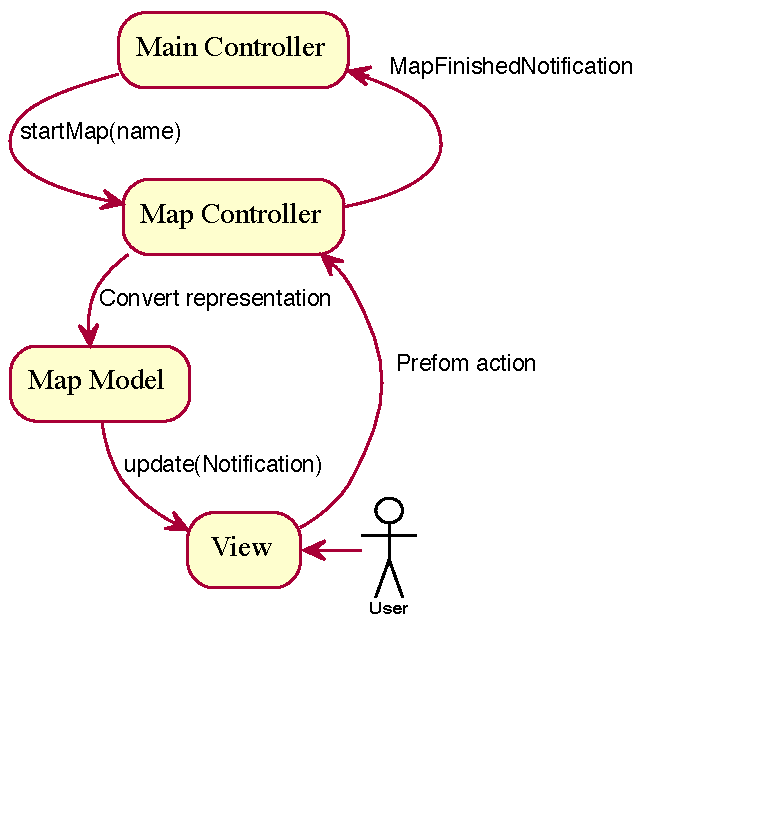
\includegraphics{figures/engine_exported.pdf}
	\caption{Overview of the implementation.}
	\label{fig:overview_engine}
\end{figure}

The system is structures using MVC for the overall architecture as well as  using the Observer Patten as shown above.
%TODO explain  mvc and Observer Patten somewhere

The \texttt{MainController} handles the overall logic, including the game progression. 
Although the objectives only required a isometric  map view, the implementation was designed to be more general  hence a \emph{separate} controller for each \texttt{stage} of the game is used. When the \texttt{stage} is finished  (e.g. when a map has been completed) the controller notifies the \texttt{MainController}, which decides what to do next.   

%TODO where to put this
%The architecture could be easily extended to overworld maps, cut-scenes for example.


The observable components (i.e. the view, and the map controller) communicate using \texttt{notification} objects which encapsulate any relevant information. For example the \texttt{model} sends a \texttt{UnitMovedNotification} when the computer controlled opponent move ones of their units. This notification includes a reference to the unit moved as well as the path it took to to get there. This information is used by the GUI to display an animation of the unit moving to the user.

\clearpage
\subsection{Data Format}
The schema for the data format was only slightly changed for the reason stated in section \ref{ssub:intercompatibility}. To parse and serialisation the xml the \texttt{Xstream} Java library was used.

XStream is an open source library used to serialise Java objects to and from XML. One of the it major benefits is that it abstracts over the parsing and serialisation and allows the user to focus on what the data should be used for. 

XStream achieves this though the use of Java annotations\footnote{A special form of syntactic metadata that can be added to source of a Java file, with the notable feature of being retained in the complied class files.}, as shown in the below example\footnote{Getter, Setters and trivial constructor omitted.}.

\begin{lstlisting}[caption=Example of class that is serialisable with XStream, label=lst:SavedTile, language=java] %Java
	
@XStreamAlias("tile")
public class SavedTile {
	protected final String type;
	protected final int height; 
	protected int startingHeight;
	
	@XStreamAsAttribute
	protected final int x;
	@XStreamAsAttribute
	protected final int y;

	protected Orientation orientation;
	protected String leftWall, rightWall;
	
	private Object readResolve() {
		if (orientation == null)  
			orientation = Orientation.TO_EAST;
		if (startingHeight == 0 && height != 0) startingHeight = height;
		return this;
	}}
\end{lstlisting}

As shown above no extra logic apart from the annotations is need for serialisation.  Another benefit of XStream is that it allows setting default values. This allows the user to omit redundant tags, as shown in the xml where most of the tags have been omitted.
\begin{lst:tile}[caption=Serialised form of the above class. ]
<tile x="0" y="0">
	<type>grass</type>
	<height>1</height>
</tile>
\end{lst:tile}

%TODO Ref

\subsubsection{Resources}

All resources that loaded are \texttt{Identifiable}, that is they have a unique id.  There are two main advantage to using this scheme. The first is that it allows caching of resources which means that there's single instance for each resource (such as weapons and images). This is especially important for the images, to reduce the memory requirements as well as the load times.

The other advantage is that it meant I could use the same framework for loading and saving all the resources, hence saving development time as well as reducing code duplication. 

A detail description of the structure and  required resource of a project is in appendix \ref{sec:project_structure___specification}.

\subsubsection{Sprite Sheets}
\label{ssub:sprite_sheets}


A sprite sheet is a collection of images combined together. The advantage of this is that a single image is loaded, which reduces loading times. It also make it easier to cache images, since a \emph{subimage} can be efficient created\footnote{using the Java method \texttt{BufferedImage.getSubimage}}. A \texttt{subimage} shares the same image data as original so it is an ideal way for each tile to have access to it's images\cite{bufferedImage}.    

\begin{figure}[htbp]
	\centering
		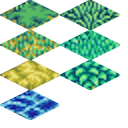
\includegraphics{figures/tileset.png}
	\caption{A 128\*128 sprite sheet containing a tileset for a map}
	\label{fig:figures_tileset}
\end{figure}

Sprite sheets make maps more reusable, since the tileset can be changed without any consequences\footnote{As long as the new tileset has the same number of image or the \texttt{tilemapping} has entries for missing images.}.  

I created a sprite sheet editor to allow the user to easily edit the tilesets. Using sprite sheets allowed abstracting over the file system, hence increasing the usability of system. The editor was reused for editing other images such as the character images and can even be used independently.
%TODO real word?

\clearpage
\subsection{Engine Development}
\label{sub:engine_development_and_testing}
\subsubsection{Map}
\label{ssub:maps}


The \texttt{Map} class handles the overall logic and game flow.   The main components are:
\begin{itemize}
\item The tiles for the maps. Each tile includes height information as well as the tile's location, as shown in listing \ref{lst:SavedTile}.

\item The enemy units.     

\item The \texttt{TileMapping} which specify what images to use in addition to \emph{how} the tile is drawn. 

\item  The \texttt{conditions} of the maps. These include a winning conditions (such as ``Defeat All Enemy Units'',  the placement of player's units and a \texttt{turnComparator} which decides how the turn ordering works.  

\item  The \texttt{events}. These include the dialog which displays parts of the story at the start and end of each battle. 
\end{itemize}

The other major responsibly of the map is to send notifications to the view.  
%TODO more

\subsubsection{Units}
\label{ssub:units}
A \texttt{unit} has set of attributes whose values can be specified by the user. A unit is the abstract representation and is storage.  A \texttt{MapUnit} extends the units sets of attributes with extra information such the location and the current hit points.

A unit has a  specified weapon (as discussed in section \ref{sub:weapons___skills}).  A weapon has a \emph{attack range} which specified how the unit attacks.  As a example consider a spear which attacks all units in a specified direction and a bow which attack a single faraway target. A unit with same attributes would play very differently with either of examples since a spear can be only used in melee combat, whereas a bow can only be used from a distance.

A unit has a set of skill (as descried in section \ref{sub:weapons___skills}). The main difference apart possibility of having \emph{multiple} skills is the concept of an \texttt{attack area}.  The \emph{attack area} is tile that are effect by the skill, which includes \emph{both} friendly and enemy units. A skill can either include the caster in the area or explicitly exclude the caster, which gives the user more flexibility.

While default implementation of skills and weapons are provided, the advance user can create their user using the extension mechanism of the data format (see section \ref{sub:data_format_extension_mechanism}).

\begin{figure}[htbp]
	\centering
 		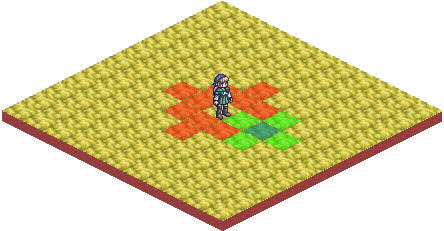
\includegraphics[scale=0.5]{figures/skill.png}
	\caption{A example of a Skill. The red squares are the \emph{attack range}, the green the \emph{attack area}}
	\label{fig:figures_engine_Skills}
\end{figure}

Units can ``level up'' which means the attributes  of the unit increase.  Levelling up can also effect how quicker the unit can get their turn. How level up is defined in the battle system as discussed in section \ref{ssub:battle_system}.

% \subsubsection{Algorithms}
% \label{ssub:Algorithms}

\subsubsection{Movement and Path Finding}

To find movement range movement range of unit Dijkstra's algorithm was used. Dijkstra's algorithm finds the shortest path from a tile to each other tile. This is of course expensive as the map is large so as a improvement I only searched \emph{locally}. Since a unit can movement at most \emph{n} squares in any direction (\emph{n} being the square the unit is allowed to move) there is no point check any tile which which is more then \emph{n} squares away.  Searching \emph{locally} means not finding the paths to any \texttt{tile} which is more then \texttt{n} squares are away.

The path are then used to display \emph{animated} unit movement to the user.  This required keeping track of the \emph{direction} in the movement algorithm. 

\def\astar{A$^{\star}$ }

Other algorithm such as \astar (which is generally an improvement for Dijkstra) was considered for finding the shortest path between two tiles. \astar was rejected since it does  provide much improvement since the paths to \emph{every} tile in range is needed. Since the paths were cached the difference would negavaitble and hence was not worth the time implementing and testing it.


\subsubsection{AI Behaviour}
Each has AI unit has a \emph{Behaviour} which specifies how the unit acts and which of the player's unit to target.  The engine provides a default implementations which try to get as close as possible to target while attacking any of the player's units that happen to be in range to be on the way.  The targets the engine provides by default include attacking the player's unit that has the lowest hp and attacking the unit with highest strength. Like other parts of the engine a user can user can provide their own behaviour to further customised by linking their classes.

\subsubsection{Turn Ordering}
The engine provides dynamic unit ordering.  This allows the ordering to change based on units attributes or actions.  The default implementation allows the unit with highest \texttt{speed} to move first.  To make the ordering more interesting it also takes account the unit's action when deciding which is the next unit to move. For example if the unit does not move (i.e. uses \texttt{wait}) they get their next turn quicker. As with other parts of the engine the user can uses their classes to further customise the unit ordering.

\subsubsection{Battle System}
\label{ssub:battle_system}

The battle system controls how units interact with each other.  It specify how damage is calculated as any affects results from an action. The engine provides a default implementation where 
\begin{itemize}
	\item The damage taken by a weapon is calculated by adding the weapons power to unit's strength and subtracting the opponent defence. The lowest a weapon can do is zero, i.e. negative damage is not allowed.
	\item The damage done by a skill is independent of the unit's attributes.
\end{itemize}

The damage done by a weapon is also affected by difference in height of the attack tile and target's tile. Attacking was a higher height gives a bonus whereas attacking was below reduces the attack.


The battle system also defines how units ``level up''. The default implementation levels up a unit when they gain 100 experience points. The unit gain experience points by perform actions. Each action gives a different amount of experience point ranging from none from using \texttt{wait} to 60 (before any modifiers are applied).

The amount of experienced gained is dependant on level on the attacker and the target. Attack a higher level unit gives a bonus whereas attacking a lower level unit reduces the amount of experienced points gained.

\subsubsection{Conditions}
\label{ssub:events}

A map has a win condition which can be specified by the user.  The engine provides two default implementation, defeat all enemy units and defeat a specific unit.  The user can of course provide their own conditions which can be basically anything e.g. move to a specific tile. 

% TODO add losing conditions to future work

\subsubsection{Dialog}
\label{ssub:dialog}
The engine supports displaying dialog to the user at the start and end of a battle. 

\begin{figure}[htbp]
	\centering
		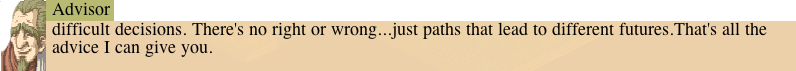
\includegraphics[width=6.3in]{figures/dialog2.png}
	\caption{A example of a dialog}
	\label{fig:figures_dialog2}
\end{figure}

One of the major features is that is that the engine handles line wrapping and pagination of the text which is in contrast to many earlier games. This allows the user to focus on writing the plot of game rather then on fitting the text into the dialog box. 

Optionally a speaker can be specified for the dialog, this can be used to have a conversation between characters on a map, to make the dialog more interactive. 

The editor as discussed in section \ref{ssub:dialog_editing} supports editing of the dialog. It has the notable features of allowing the user to visually reorder parts of the dialog. It also supports   importing and exporting the dialog as a text file.  This allows the user to write the script of the game independently in whatever application they prefer. 


\subsection{Saving and Loading}
The engine supports Saving and Loading at any point during the game. The only possible downside  for the user is that when the the saved data is loaded, game continues from the \emph{beginning} of the map which was lasted played. 

The reason for this limitation is to keep the save format small and easy to load. Using this methods means the only details that need to be saved are the maps left to be played and units attributes (which can change since units can ``level up''). 

The other limitation is that there only one save file. This not as big limitation as it seems since the the save file is stored in users home directory, meaning each user would have their own save.

\subsection{Inter-compatibility}
\label{ssub:intercompatibility}
As discussed previously the maps use xml as their data format, one the advantages of this was that it required very little changes to the data format to have incompatibility with Oleksandr Stasyk's  Terrain Generator's output format.  The Terrain generator allows uses various algorithms to produce a sensible looking map. Users can use these maps as a starting point for their own creation, hence lowers the time and effort to design a map.

The terrain generator is called by the editor on behalf on the user with appropriate settings\footnote{In the form of a YAML configuration file \texttt{bundle/config.yaml}} saving the user from having to configure the many options available in the terrain generator (since the terrain generator is a command line application).

% \subsection{GUI Development and Testing}

\subsection{Map Rendering}
\label{ssub:map_rendering}

The GUI uses isometric viewpoint to display the map. 
%TODO more

\begin{figure}[htbp]
	\centering
		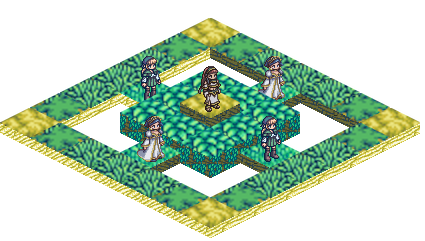
\includegraphics[height=3in]{figures/imp-map.png}
	\caption{A isometric map which shows the features of the renderers including height, empty tiles, wall textures and unit placement}
	\label{fig:figures_imp-map}
\end{figure}

The map is composed of isometric tiles which have the following features:

\begin{itemize}[topsep=0mm,noitemsep ]
	\item  The height is \emph{exactly} halve the tile's width.
	\item  To create the tile, a square tile is rotated by 45$^{\circ}$ then height is halved.
\end{itemize}

One the major features of the map render is how the height is specified.  Instead of using a bunch of careful constructed tiles to simulate height, each tile has a specified height which the renderer uses to draw the tile with appropriate height. 

\subsubsection{Drawing Algorithm}
The algorithm for drawing tiles, first the top of the tile is drawn, then the walls are drawn. It quite general since it supports tiles which can slant in any direction as shown in figure \ref{fig:mtile2} where the tile is slanting to the north as well as zooming and arbitrary height \footnote{A simulate of the equations was made first and is in \texttt{IsomerticRendering.gcx} (Mac Only).}. 

\def\tileSize{3in}
\begin{figure}[h!tbp]
	\begin{center}
	\subfigure[A Tile with  a height 2]{
		\label{fig:mtile1} 
\includegraphics[width=\tileSize]{figures/tile1.png}} 
	\subfigure[A Tile with a start height 1 and an end height of 2 with the walls in green and red]{
		\label{fig:mtile2} 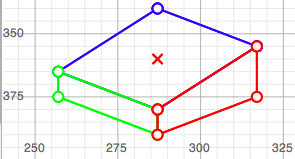
\includegraphics[width=\tileSize]{figures/tile3.png}} 
	\caption{The above figure shows normal and slanted tiles, The red X is the start point for drawing}
	\label{fig:mtile0}
	\end{center}
\end{figure}

Mathematically the set of points used to draw tile are as follows:
\begin{equation}
\; \left[ \begin{array}{c} x \\ y \end{array} \right]=\left\{ \left[ \begin{array}{c} tx \\ ty-h2 \end{array} \right],\left[ \begin{array}{c} tx+\frac{hoz}{2} \\ ty-h2+\frac{vet}{2} \end{array} \right],\left[ \begin{array}{c} tx \\ ty-h1+vet \end{array} \right],\left[ \begin{array}{c} tx-\frac{hoz}{2} \\ ty-h1+\frac{vet}{2} \end{array} \right] \right\}
\end{equation}

\begin{equation}
\; \left[ \begin{array}{c} x \\ y \end{array} \right]=\left\{ \left[ \begin{array}{c} tx \\ ty-h2 \end{array} \right],\left[ \begin{array}{c} tx+\frac{hoz}{2} \\ ty-h2+\frac{vet}{2} \end{array} \right],\left[ \begin{array}{c} tx \\ ty-h1+vet \end{array} \right],\left[ \begin{array}{c} tx-\frac{hoz}{2} \\ ty-h1+\frac{vet}{2} \end{array} \right]\right\}
\end{equation}

\begin{equation}
\hspace{-2.5cm} \left[ \begin{array}{c} x \\ y \end{array} \right]=\left\{ \left[ \begin{array}{c} tx \\ ty-h1+vet \end{array} \right],\left[ \begin{array}{c} tx-\frac{hoz}{2} \\ ty-h1+\frac{vet}{2} \end{array} \right],\left[ \begin{array}{c} tx-\frac{hoz}{2} \\ ty+\frac{vet}{2} \end{array} \right],\left[ \begin{array}{c} tx \\ ty+vet \end{array} \right] \right\}
\end{equation}

\begin{align*}
	tx,\; ty   &\;\; \textrm{are the start point (shows an red X in the above figure)}\\
	vet,\; hoz &\;\; \textrm{is the height and width of the tile adjusted for  the zoom and pitch}\\
	h1,\; h2   &\;\; \textrm{are difference in the start height and end height and via verse}
\end{align*}

where equation 1, is for the top of the tile, equation 2 for the right wall and equation 3 for the right wall. 

The equation converted to Java easily since the \texttt{Graphic} class has the methods  \texttt{drawPolygon} which draw a polygon using set of points conveniently in same form as the equations.

%TODO
\subsubsection{Images and Texture Mapping}
The top of tile can be texture mapped or be drawn directly from an image.  Texture mapping repeats a usually small image across the tile. This is the simpler method for the user since they only have to provide a small texture image, but they loss control over where exactly the image is drawn.  Texture mapping is also required for slanted tiles since too many variations to provide image for,

The user also has the option of use a image which is drawn directly. To do this the would have to provide their own isometric tile\footnote{There are script to help the user though}. This methods allows more control on whats drawn.  

Walls like slanted tiles are always texture mapped since they to many variations to provide images for. 

\subsubsection{Units}
Each image has at minimum \emph{four} images associated it, for each direction (east, west, north, south). These are used to show which way the unit is facing. The unit can also has a animation with each direction,to making unit movement more interactive. The unit can also optionally has a portrait which if available would be used for their dialog.

\subsubsection{Reusability}
Since the map renderer is not dependant on Main GUI, it could be reused in many different places in the editor. 

\subsection{Map Rotation}
The map renderer supports for different rotations which the user can choose from. This is implementation \emph{not} by actually rotating the map (since this would be Expensive) but by changing the draw order. By default (0,0) is on the top left of the map. Rotation mealy changes the location of (0,0). This means that none of the tile have changed so all the cached calculations can be kept. 

Rotating the map can be used by the user to see units that are hidden or obstructed by tiles. 

\clearpage
\subsection{User Interface}
\subsubsection{Controls}
The main control scheme for the GUI, but the user can perform nearly every action using the mouse. All the elements were designed to work equally well with the mouse and keyboard. This means for example that the tiles are clickable, (which result in tile being selected when clicked).  

%TODO talking about unit clicking

\subsubsection{Menus}

The GUI uses a menu system to handle the units actions. The menu is quite general since it will resize to the longest item in the menu.  It also supports nested menus which are used when user chooses to use a skill. The menu is controllable using the keyboard using the arrows keys, the user can also click a item directory to select it.

% TODO FSM enum


\subsubsection{Other Features}
The GUI supports of other features to improve the user experience these including

\begin{itemize}
	\item Zoom in/out which lets the user see more detail. 
	\item Changing the \texttt{pitch} of the map (increasing the pitch flattens the map which allows the user to easily see obstructed units).
	\item A \texttt{log} which can be used to see which actions have taken place. Useful to find out what the enemy has done if the user miss it the first time.
	\item The key mapping is displayed to user on startup.
	\item The GUI automatically scroll to enemy unit's location if they are out of range when it is there turn.
	\item The unit information shows the unit's attributes include the current hit points. They are are displayed in different colour for opposing units to easily distinguished them. 
\end{itemize}


\subsection{Editor Development}
%TODO finish

\subsubsection{Overview}
\label{ssub:overview}

The editor allows the user to customise nearly all aspects of the engine.  Notable features include visual map making as was exporting the created game as a completely self contained application with \emph{no} external dependencies apart from a recent version of Java\footnote{specify Java 6+}. 

The editor uses a tabbed interface, the benefit of is that it shows the users whats available in the editor. Each tab has share the same overall structure, for two reason, namely to keep the all aspect of the editor consistent hence making it easer it to use. The second reason is that, most of the code can be reused for each tab saving development time. 

In each tab the of current resources created is listed on the left as shown in figure \ref{fig:figures_editor_Units}. The user can click on any of the resources to customise them. At the bottom of the list are two button the left button (--) removes the selected resource whereas the right button (+) add new resource. Since it is likely the user would create simpler resources (e.g  weapon of the same type differing only in Strength) any new created resource takes on the characteristics of last selected item.

\begin{figure}[htbp]
	\centering
		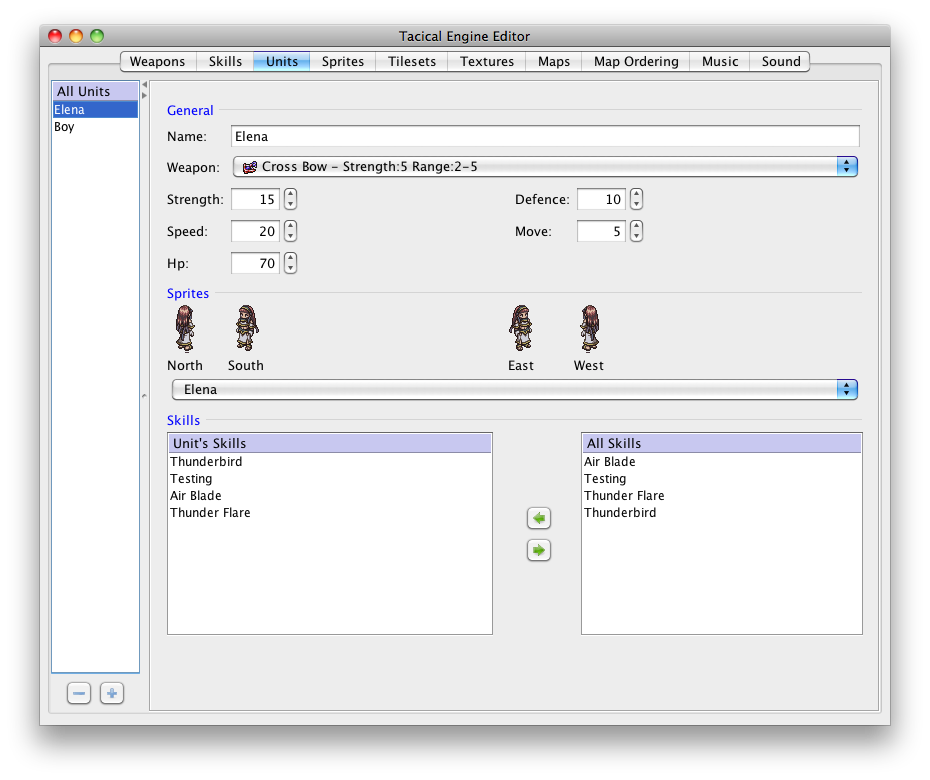
\includegraphics[width=\textwidth]{figures/editor/Units.png}
	\caption{Unit Editor}
	\label{fig:figures_editor_Units}
\end{figure}


To prevent error and increase usability,  \texttt{JSpinner} were used wherever numeric input was needed. \texttt{JSpinner} allows a minimum and maximum range to be specified,  the component will then reject any input which is not in range.

Each of tab can use the data from other tabs, as shown above where the weapons and skills are received. One of the advantages is the data is always consistent. This was made a lot simpler since the user can only edit one set of resources at a time.

\clearpage
\subsubsection{Weapons \& Skills}

The editor support customising the weapons and skills as shown. 

\def\editor{0.237}
\begin{figure}[htbp]
	\begin{center}
	\subfigure[Weapons Panel]{
		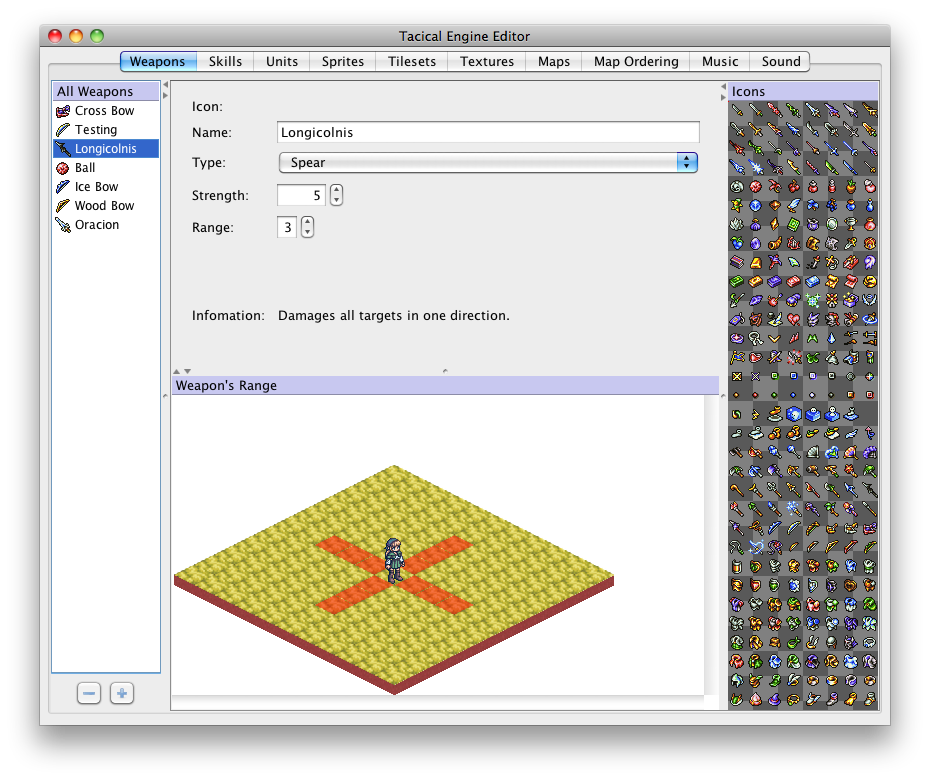
\includegraphics[scale=\editor]{figures/editor/Weapons.png}}
	\subfigure[Skill Panel]{
			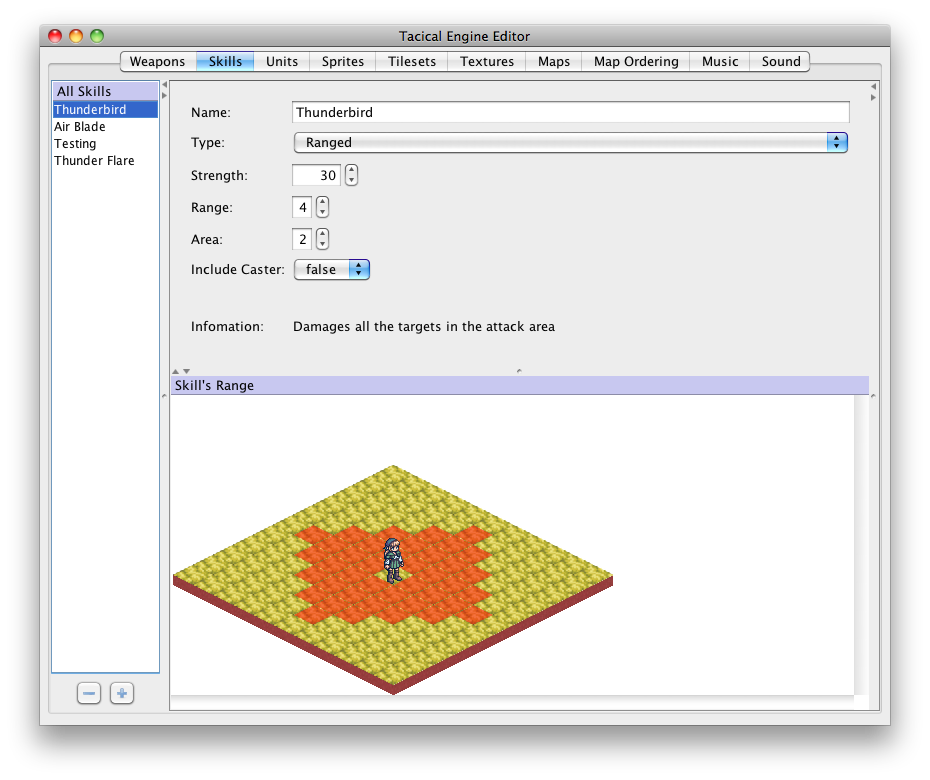
\includegraphics[scale=\editor]{figures/editor/Skills.png}}
	\end{center}
	\label{fig:editor}
\end{figure}

The editor shows visually what the attack range looks like. This is updated whenever the user make any change to the resource.  This required very little extra code since the map renderer was general enough to be easily embedded. 

\subsubsection{Unit Editor}
\label{ssub:unit_editors}
The unit allows the user to edit all that attributes of the units. These include the skills, weapon as well as the images unit as shown in figure \ref{fig:figures_editor_Units}. 


\subsubsection{Sprite Sheet Editor}
Sprite sheet editor are used for many of the tabs including the Units's image, textures and tileset.
\begin{figure}[htbp]
	\centering
		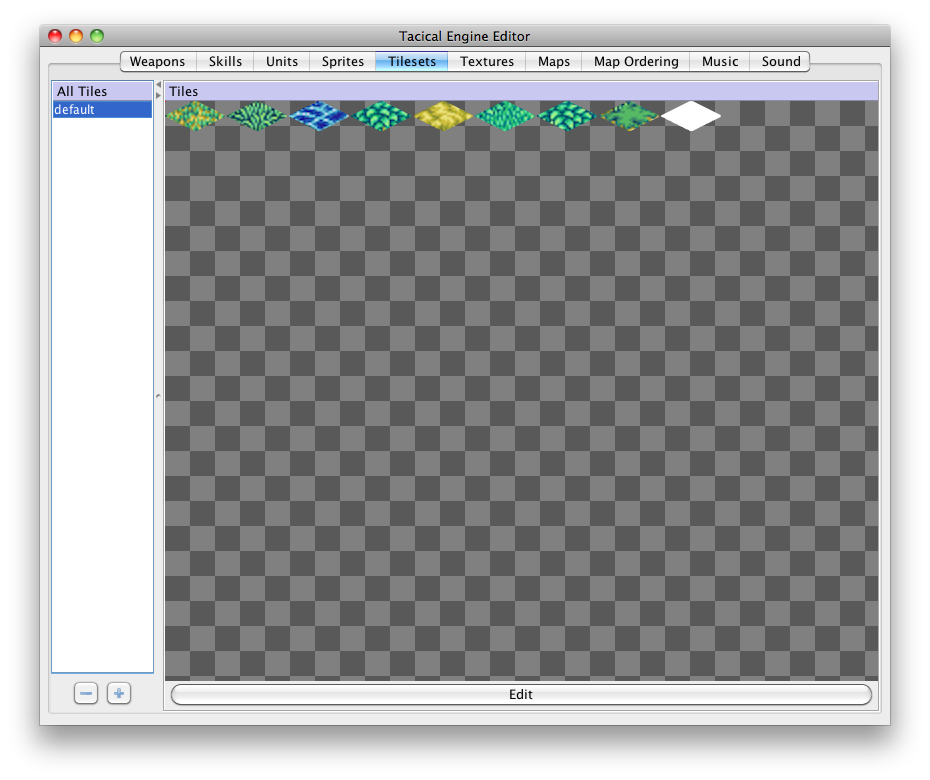
\includegraphics[width=0.75\textwidth]{figures/editor/tileset_edit.png}
	\caption{A sprite sheet  editor for the tiles}
	\label{fig:figures_editor_tileset_edit}
\end{figure}

\subsubsection{Music Editing}
\begin{figure}[htb]
	\centering
		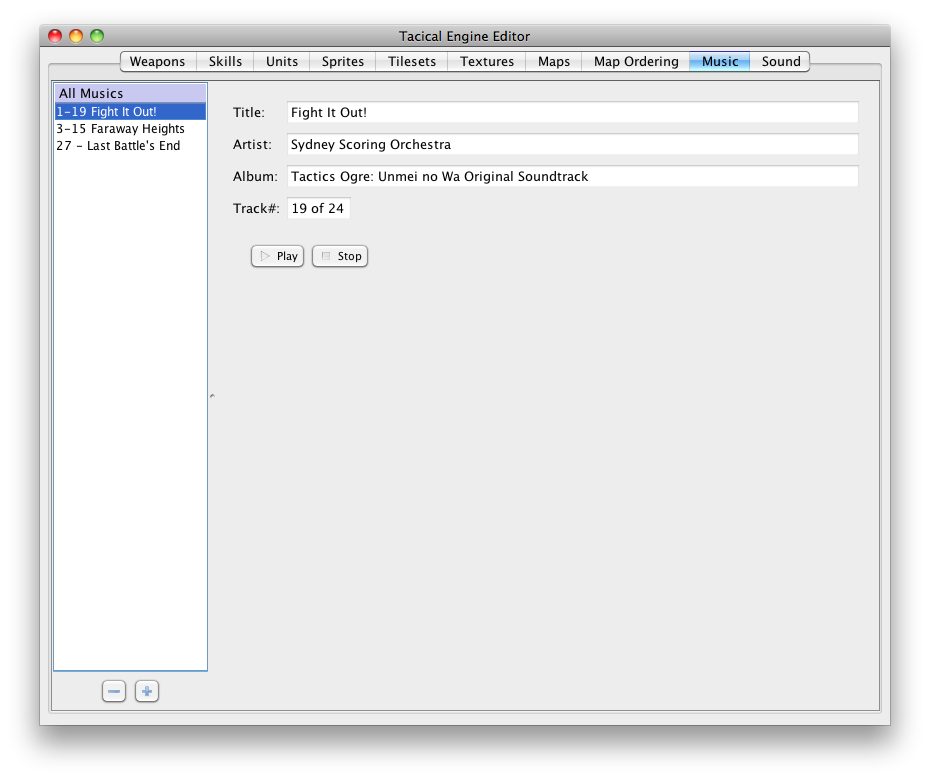
\includegraphics[width=0.75\textwidth]{figures/editor/Music.png}
	\caption{The Music Editor}
	\label{fig:figures_editor_Music}
\end{figure}
The music editor supports choosing which music are alviable to use in the game.  When a track is selected in the editor, the metadata (include the `artist' and `album') of the track is displayed.  As a further enhancement, the track can be previewed this especially useful when used in combination with the  sound effect editor (which has exactly the same interface) to see what the combination of sounds and music sound like. 

\clearpage

\subsubsection{Visual Map editing}
%TODO finish
%TODO deferfed map

\clearpage
\subsubsection{Dialog Editing}
\label{ssub:dialog_editing}

\begin{figure}[htbp]
	\centering1
		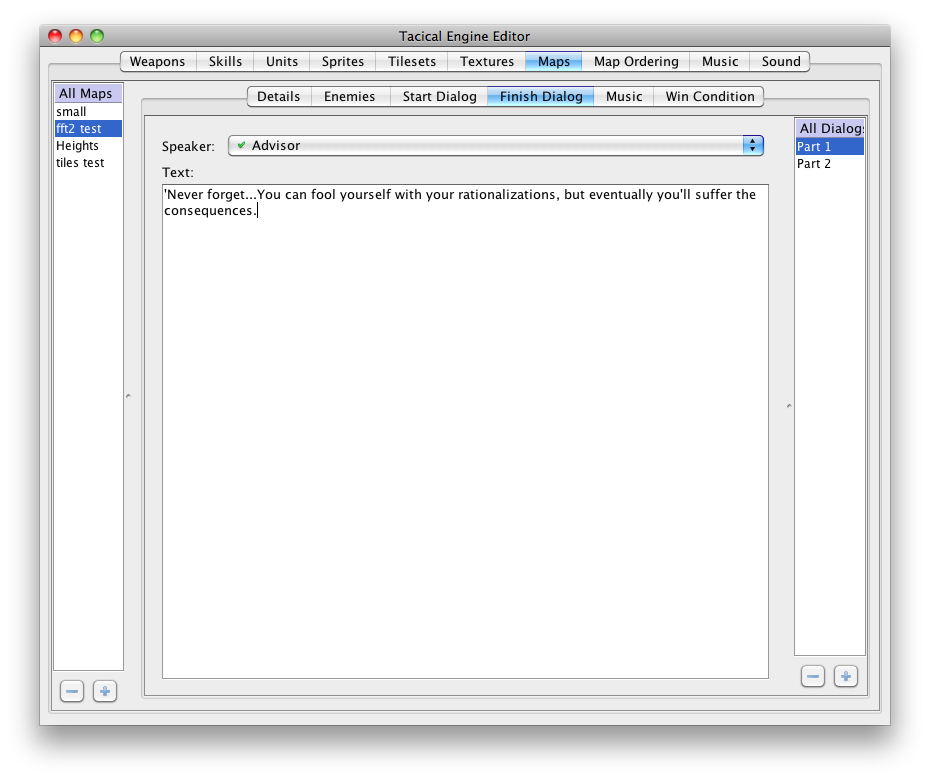
\includegraphics[height=4in]{figures/editor/Maps-dialog.png}
	\caption{The dialog editing panel}
	\label{fig:figures_editor_Maps-dialog}
\end{figure}
The editor supports the creation of dialog.  A dialog is sequential of parts. Each part has the text  associated with it as well optionally have a speaker.  The speaker can be selected from any unit that is already been placed on the map. This a vast improvement on the original design where the user types the name of the speaker since less change of making errors. \footnote{It would also cause runtime exceptions if there was no unit with that name.}.

As mentioned before, the engine takes care of pagination as well line wrapping when displaying the dialog in the game. This frees the user from having to fit the text into a specified area. 

\paragraph{Import/Export\\}
The editor also supports importing as well as exporting the dialog in format shown below. 
\begin{lstlisting}[caption=Shows the format used  for the dialog]
- speaker1: Some text 
- speaker2: Some more text
- none:     This part has no speaker
\end{lstlisting}
This allows the dialog to be easily written in the user's preferred application.  This could be useful if separate person writes the dialog of the game since the person does not need a copy of the editor. The format is described in more detail in appendix \ref{ssub:dialog_data_format}  

\subsubsection{Project Selection}
\begin{figure}[htbp]
	\centering
		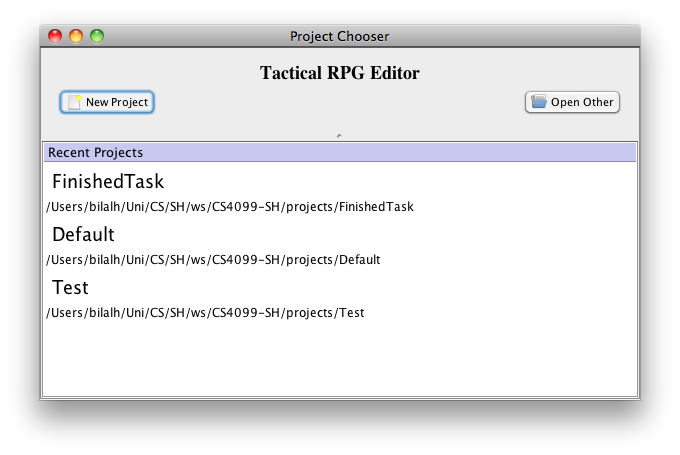
\includegraphics[width=1.05\textwidth]{figures/editor/Project_Selection.png}
	\caption{The Project Selection Window which is shown at startup}
	\label{fig:figures_editor_Project_Selection}
\end{figure}

When the editor starts It shows the above startup screen which allows the user to create a new project or open an existing project.  Since a user is likely to work on the same project for a significant period of time, the editor keeps tracks of recent projects. 

%TODO put bug when loading music stops
\clearpage
\subsubsection{Exporting}
\label{ssub:exporting}

The editor can export the game as a complete package, either as a Mac OS X application or as jar. These application don't require any external resources, apart from a recent version of Java\footnote{specifically Java 1.6+}.

A prominent feature of the editor is that the jar will work on any Java enabled platform, since the jar contains all required libraries for each platform. The OS X application can even be exported on other platforms.

While most of the testing was done on OS X \footnote{Mac OS X 10.6 Snow leopard}, it also works well on Linux \footnote{Science  Linux x.y}. It  even has limited compatibly with Windows \footnote{Tested on Windows 7 32 bit} (apart from some minor graphics issues).

\subsection{Ant Build File}
\begin{itemize}
	\item Builds the projects
	\item Runs tests
	\item Make dist versions
	\item Links Jars
\end{itemize}